\documentclass[margin = 10pt]{standalone}
\usepackage{tikz,pgfplots}
\usetikzlibrary{calc}
\pgfplotsset{
    compat = 1.18,
    every axis title/.style ={
            align=left,
            fill=yellow!20,
            inner sep=1pt,
            rounded corners=1pt,
            at={(axis description cs:0.5,1)},
            shift={(0,1cm)}
        },
    every axis grid/.style = {
        dashed,
        line width = 0.1pt,
        color = gray,
        },
}

\begin{document}
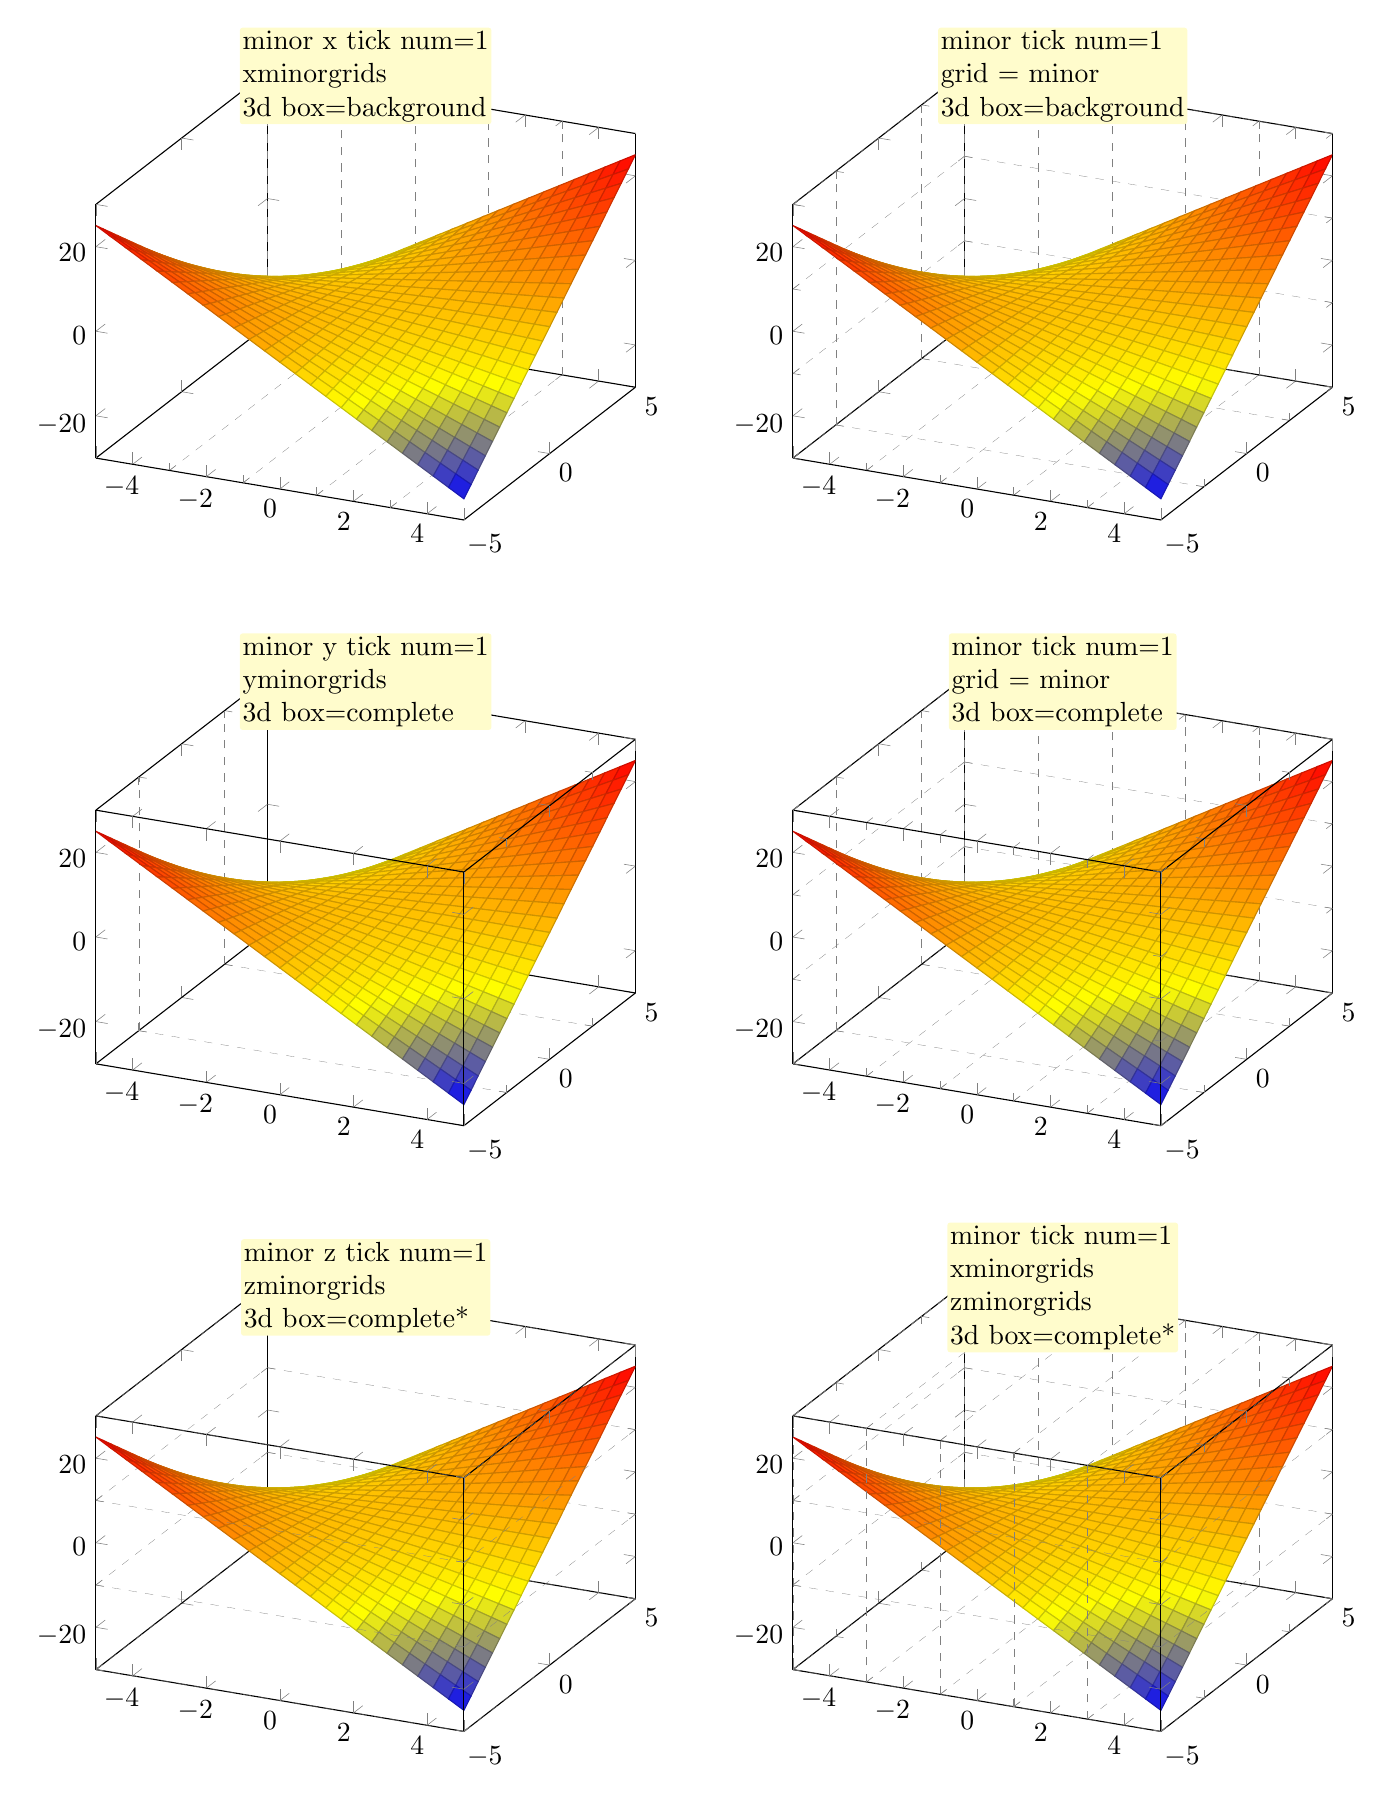
\begin{tikzpicture}
\begin{axis}[
    name= r1,
    title = {minor x tick num=1\\xminorgrids\\3d box=background},
    minor x tick num=1, 
    xminorgrids,
    3d box=background
    ]
\addplot3 [surf] {x*y};
\end{axis}

\begin{axis}[
    anchor = west,    
    at={($(r1.east)+(2cm,0)$)},
    title = {minor tick num=1\\ grid = minor\\3d box=background},
    minor tick num=1, 
    grid = minor,
    3d box=background
    ]
\addplot3 [surf] {x*y};
\end{axis}

\begin{axis}[
    name= r2,
    anchor = north,    
    at={($(r1.south)+(0cm,-2cm)$)},
    title = {minor y tick num=1\\yminorgrids\\3d box=complete},
    minor y tick num=1, 
    yminorgrids,
    3d box=complete
    ]
\addplot3 [surf] {x*y};
\end{axis}
 
\begin{axis}[
    anchor = west,    
    at={($(r2.east)+(2cm,0)$)},
    title = {minor tick num=1\\ grid = minor\\3d box=complete},
    minor tick num=1, 
    grid = minor,
    3d box=complete
    ]
\addplot3 [surf] {x*y};
\end{axis}

\begin{axis}[
    name= r3,
    anchor = north,    
    at={($(r2.south)+(0cm,-2cm)$)},
    title = {minor z tick num=1\\zminorgrids\\3d box=complete*},
    minor z tick num=1, 
    zminorgrids,
    3d box=complete*
    ]
\addplot3 [surf] {x*y};
\end{axis}

\begin{axis}[
    anchor = west,    
    at={($(r3.east)+(2cm,0)$)},
    title = {minor tick num=1\\ xminorgrids\\zminorgrids\\3d box=complete*},
    minor tick num=1, 
    xminorgrids,
    zminorgrids,
    3d box=complete*
    ]
\addplot3 [surf] {x*y};
\end{axis}

\end{tikzpicture}
\end{document}